Following the experimental process described in Section \ref{sec:sys_eval}, 120 experiments were performed 50 times each for statistical significance. This section highlights the main results from the performed experiments.

\subsection{Writing Experiments}

Figures \ref{fig:res_writing_3} and \ref{fig:res_writing_2} show the write throughput of all three pipelines defined in Section \ref{subsec:experimental_design} when writing the five different tables defined in Section \ref{subsec:dataset}. This experiment makes use of 1 \gls{CPU} core. 

Each value reported was calculated by measuring the time taken to write the table. An example consists of delta-rs on \gls{HopsFS} which took 184.12783 seconds to write 60 M rows, so dividing the rows by time the throughput obtained is 325860.566 rows/second. This result is then resampled using the bootstrapping technique, and the average, in this case, 339.288 K rows/second is obtained. A 95\% confidence interval was also calculated (in this case \textpm 5.05 K rows/second). Still, it was not displayed in the graph as it would be hardly readable as all results are out of each other's 95\% confidence interval.


\begin{figure}
    \centering
    \begin{subfigure}[b]{\textwidth}
        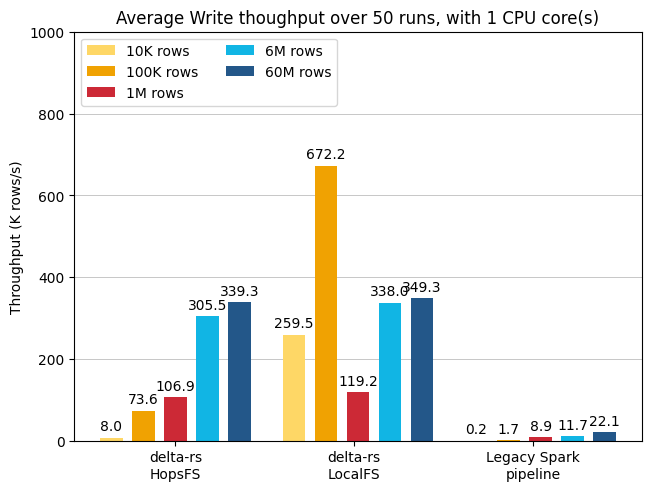
\includegraphics[width=\textwidth]{figures/5-results/diagram_three_tech_write_1_core.png}
       \caption{}
       \label{fig:res_writing_3}
    \end{subfigure}
    
    \begin{subfigure}[b]{\textwidth}
        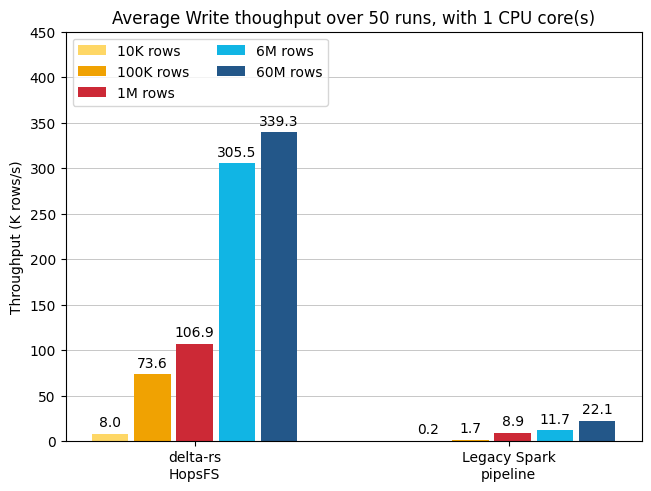
\includegraphics[width=\textwidth]{figures/5-results/diagram_two_tech_write_1_core.png}
       \caption{}
       \label{fig:res_writing_2}
    \end{subfigure}
    
    \caption{(a) Throughput for writing tables (from the TCP-H benchmark) via the three different pipelines defined in Section \ref{subsec:experimental_design}. This experiment uses 1 \gls{CPU} core.
    (b) As for (a) but showing only the legacy system and newly implemented system.}
\end{figure}

\subsection{Reading Experiments}

Figures \ref{fig:res_reading_3} and \ref{fig:res_reading_2} show the read throughput of all three pipelines defined in Section \ref{subsec:experimental_design} when writing the five different tables defined in Section \ref{subsec:dataset}. This experiment makes use of 1 \gls{CPU} core. 

Each value reported was calculated by measuring the time taken to read the table. An example consists of delta-rs on \gls{HopsFS} which took 0.0378069 seconds to read 60 M rows, so dividing the rows by time the throughput obtained is 1587.0114 M rows/second. This result is then resampled using the bootstrapping technique, and the average, in this case, 1929.861 M rows/second is obtained. A 95\% confidence interval was also calculated (in this case \textpm 102.7 M rows/second). Still, it was not displayed in the graph as it would be hardly readable as all results are out of each other's 95\% confidence interval.

\begin{figure}
    \centering
    \begin{subfigure}[b]{\textwidth}
        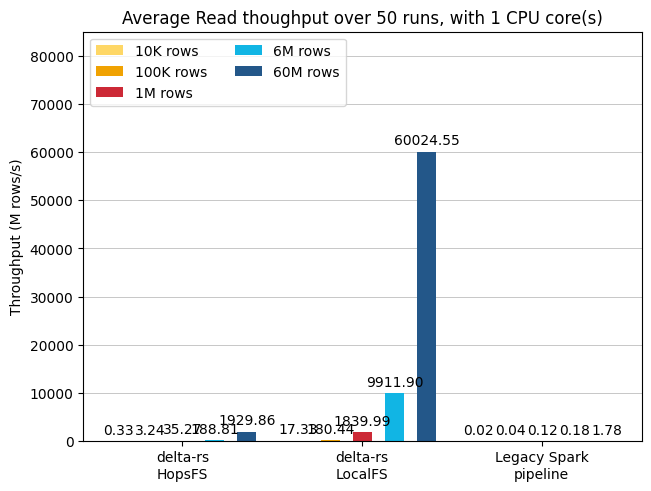
\includegraphics[width=\textwidth]{figures/5-results/diagram_three_tech_read_1_core.png}
       \caption{}
       \label{fig:res_reading_3}
    \end{subfigure}
    
    \begin{subfigure}[b]{\textwidth}
        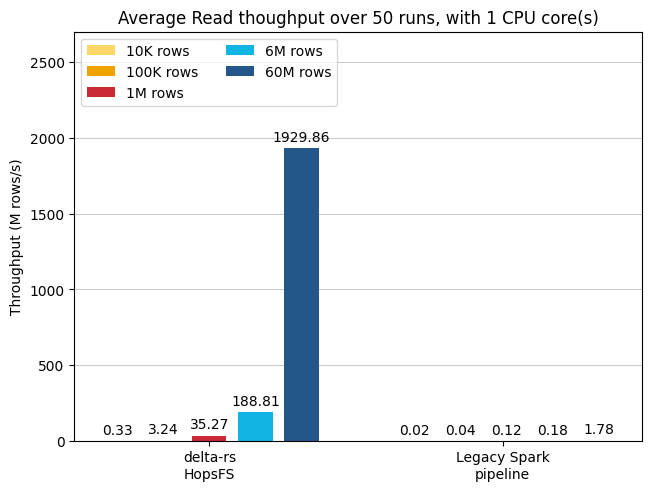
\includegraphics[width=\textwidth]{figures/5-results/diagram_two_tech_read_1_core.png}
       \caption{}
       \label{fig:res_reading_2}
    \end{subfigure}
    
    \caption{(a) Throughput for reading tables (from the TCP-H benchmark) via the three different pipelines defined in Section \ref{subsec:experimental_design}. This experiment uses 1 \gls{CPU} core.
    (b) As for (a) but showing only the legacy system and newly implemented system.}
\end{figure}

\subsection{Experiments with more \glsfmtshort{CPU} cores}

Experiments reading and writing tables from the TPC-H benchmark in the three different pipelines defined in Section \ref{subsec:experimental_design} were repeated with increasingly more \gls{CPU} cores. The Tables \ref{tbl:cpu_percent_diff_write} and \ref{tbl:cpu_percent_diff_read} display the percentage increase between the first and the increased \gls{CPU} cores experiment. For example, the delta-rs \gls{HopsFS} pipeline throughput when writing a 60M rows table is 339.288979358 k rows/second, when using 1 \gls{CPU} core. During the experiment using 8 \gls{CPU} cores the throughput was 494.7344718446817 k rows/second. Thus, the throughput performance increase as a percentage is 45.82 \% (calculated as the rate between the increase and the 1 \gls{CPU} experiment multiplied by 100). Note that in some cases the performance increase is negative, meaning that the throughput decreased even if computational resources were increased.

\begin{table}
    \centering
    \begin{subtable}[t]{\textwidth}
        \begin{tabular}{c c c c c c} 
            \toprule
            Pipeline\Tstrut\Bstrut & \thead{Rows \\ number} & \thead{1 CPU core throughput \\ (k rows/second)} & \thead{2 CPU cores\\ (\% increase)} & \thead{4 CPU cores\\ (\% increase)} & \thead{8 CPU cores\\ (\% increase)} \\
            \midrule
            \multirow{5}{4em}{delta-rs\\ HopsFS} & 10K & 8.005477660 & -0.94 & 2.87 & -2.37\\ 
            & 100K & 73.550934236 & 4.77 & 1.89 & 5.88\\ 
            & 1M & 106.932925730 & 10.41 & 11.69 & 13.20\\
            & 6M & 305.503687034 & 21.39 & 21.93 & 26.17\\
            & 60M & 339.288979358 & 32.46 & 43.43 & 45.82\\
            \midrule
            \multirow{5}{4em}{delta-rs\\ LocalFS} & 10K & 259.548165052 & -18.62 & -12.92 & -9.38\\ 
            & 100K & 672.239894235 & 9.15 & 13.83 & 10.25\\ 
            & 1M & 119.198512205 & 17.51 & 17.65 & 16.84\\
            & 6M & 338.020789871 & 17.29 & 23.20 & 25.42\\
            & 60M & 349.252743491 & 32.89 & 42.35 & 43.81\\
            \midrule
            \multirow{5}{4em}{Legacy \\ Spark} & 10K & 0.199571379 & -1.03 & -2.09 & -1.99\\ 
            & 100K & 1.681863191 & -0.35 & 0.04 & -1.28\\ 
            & 1M & 8.922017340 & 3.28 & 3.04 & 2.48\\
            & 6M & 11.722915952	& 8.13 & 6.19 & 7.56\\
            & 60M & 22.099807565 & 15.99 & 15.75 & 16.78\\
            \bottomrule
        \end{tabular}
        \caption{Writing Experiment}
        \label{tbl:cpu_percent_diff_write}
    \end{subtable}

    \begin{subtable}[t]{\textwidth}
        \begin{tabular}{c c c c c c} 
            \toprule
            Pipeline\Tstrut\Bstrut & \thead{Rows \\ number} & \thead{1 CPU core throughput \\ (M rows/second)} & \thead{2 CPU cores\\ (\% increase)} & \thead{4 CPU cores\\ (\% increase)} & \thead{8 CPU cores\\ (\% increase)} \\
            \midrule
            \multirow{5}{4em}{delta-rs\\ HopsFS} & 10K & 0.3316539 & -3.12 & 11.85 & 1.10\\ 
            & 100K & 3.237530 & 14.15 & 9.27 & 17.28\\ 
            & 1M & 35.26714	& -1.87 & -5.09 & -4.15\\
            & 6M & 188.8125 & 9.35 & 8.21 & 11.75\\
            & 60M & 1929.861 & 2.03	& 6.53 & -1.90\\
            \midrule
            \multirow{5}{4em}{delta-rs\\ LocalFS} & 10K & 17.32663 & 3.40 & 8.11 & 1.33\\ 
            & 100K & 180.4406 & 1.75 & 0.10 & -5.01\\ 
            & 1M & 1839.990	& -6.14 & 2.36 & -5.58\\
            & 6M & 9911.899 & -0.06 & -2.35 & -6.69\\
            & 60M & 60024.55 & 29.03 & 17.94 & 7.89\\
            \midrule
            \multirow{5}{4em}{Legacy \\ Spark} & 10K & 0.01586513 & 0.90 & -0.12 & 0.57\\ 
            & 100K & 0.03773604 & -0.49 & 0.39 & -0.44\\ 
            & 1M & 0.1176966 & 0.27 & -2.10	& 2.71\\
            & 6M & 0.1791499 & 0.42 & 0.22 & 0.25\\
            & 60M & 1.783280 & 0.11	& 0.11 & 1.62\\
            \bottomrule
        \end{tabular}
        \caption{Reading Experiment}
        \label{tbl:cpu_percent_diff_read}
    \end{subtable}
    \caption{(a) Table showing the percentage increase in the throughput during the writing experiment with the increase of \gls{CPU} cores allocated. Experiments are indicated for each table and pipeline defined in Section \ref{subsec:experimental_design}. The throughput of the 1 \gls{CPU} writing experiment is reported for reference.
    (b) As for (a) but for the reading experiment.}
\end{table}

\subsection{Writing using legacy Spark pipeline -- Time breakdown}

During the writing experiment performed using the legacy Spark pipeline the contribution of different parts of the process were measured: namely the upload time and materialization time, dichotomy explained in Section \todo[inline]{Ref here time breakdown expl.}. This served to verify how different parts of the legacy pipeline scaled with table sizes, and if Spark was the bottleneck of the architecture.

\begin{figure}[!ht]
    \centering
    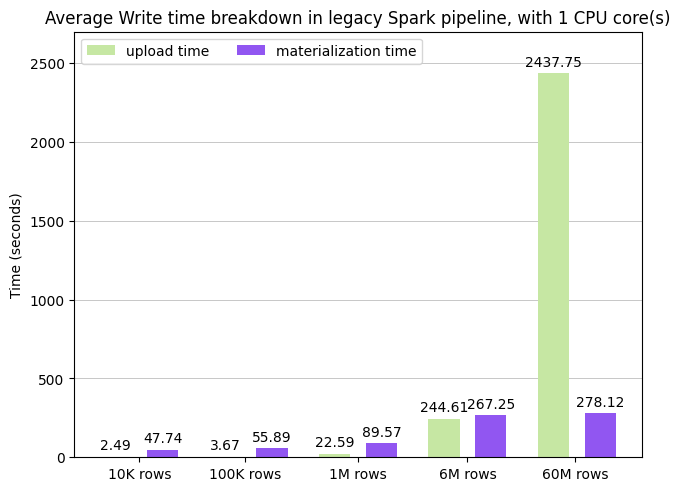
\includegraphics[width=\textwidth]{figures/5-results/diagram_hudi_virtualiz_1_core.png}
    \caption{Breakdown of the time contribution to the time needed to execute a write operation on the legacy Spark pipeline. To know more about the legacy Spark pipeline and the upload-materialize dichotomy refer to Section \todo[inline]{ref to background explaining}}
    \label{fig:hudi_virtualiz_breakdown}
\end{figure}